\section{Hyperparameter Optimization}\label{subsec:hyperparameters}

There are five hyperparameters that affect the performance of \textit{SPIND}. These include the size of the initially generated chunks (\textit{CHUNK\_SIZE}), the maximum number of values retained in main memory during the sorting phase (\textit{SORT\_SIZE}), the maximum number of files merged simultaneously (\textit{MERGE\_SIZE}), the total queue size across all relations during candidate validation (\textit{VALIDATION\_SIZE}), and the level of parallelization (\textit{PARALLELISM}) in all phases of the execution. Using Bayesian optimization \cite{shahriari2015taking}, we iteratively identify parameter configurations that minimize \textit{SPIND}'s execution time across datasets. We set the minimum chunk size to 10,000 to prevent the creation of an excessive number of files, with a maximum limit of 100 million. During sorting, the maps are constrained between 100,000 and 50 million to strike a balance between the number of files generated and staying within the main memory limit of 20 GB. The number of files merged at the same time is restricted to a minimum of two and a maximum of 2,000 to avoid overloading the file system. The buffers for the relations during validation are capped at 1 million. Lastly, the level of parallelization is capped by the number of virtual threads available on the executing machine (twelve).

The experiments are carried out using the datasets \textit{EU}, \textit{US}, and \textit{TPC-H 1}, \textit{Population}, \textit{UniPort}. These datasets have varying structures, and optimizing the parameters for all of them at the same time will assist us in identifying robust configurations that do not overfit any specific dataset structure. 

The first observation is that the degree of \textit{PARALLELISM} has a clear negative correlation with the execution time. We find that the fastest executions use at least 9 threads, regardless of how the other four parameters are set. The subsequent observation indicates that \textit{CHUNK\_SIZE} is the second most significant hyperparameter. Although smaller chunks are directly related to the total number of files created and the associated I/O overhead, an optimal chunk size of five to seven million was identified, which is also stable for \textit{Musicbrainz}, \textit{TPC-H 10}, and \textit{UniProt}. Smaller chunk sizes allow for more parallel task processing, which demonstrates mitigation of I/O operations at a certain point.

The remaining hyperparameters are far less influential and do not show a clear pattern on their own. We establish a stable configuration with a chunk size of 6 million. Sort maps are limited to 25 million nested entries, files merged simultaneously to 1.200, validation buffers to 250,000, and parallelization to 12. The configuration will be used for the execution times shown in Table \ref{tab:runtimes}.

\begin{figure*}[!t]
    \centering
        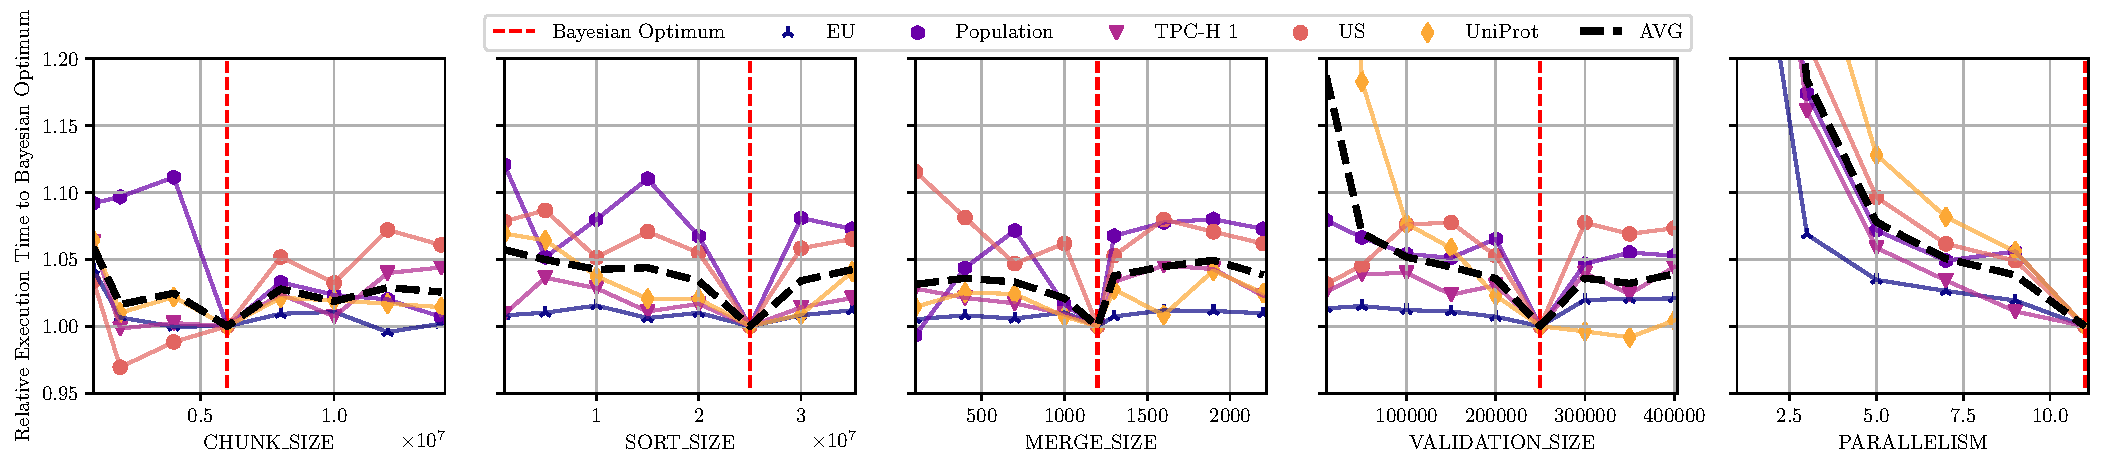
\includegraphics[width=.98\textwidth]{figures/sensitivity.pdf}
    \caption{Sensitivity around the hyperparameters obtained through Bayesian optimization}
    \label{fig:hyperparameters}
\end{figure*}

A sensitivity analysis indicated that the five parameters maintain stability close to the optimal values identified by Bayesian optimization. Figure \ref{fig:hyperparameters} presents a subplot for each hyperparameter. The x-axis represents the hyperparameter values, while the y-axis, shared between plots, depicts the relative runtime compared to the run with the Bayesian optimization settings. In the \textit{CHUNK\_SIZE} plot, it is evident that for some datasets, an alternative configuration might perform better. With more knowledge of the data set, deviating from our recommended hyperparameter settings could be beneficial.


